\begin{table}[thb]
    \centering
    \caption{各対話行為で提案手法を行った際の結果}
    \vspace{3mm}
    \label{tab:action_hikaku}
    \begin{tabular}{|c||r|r|r|r|} \hline
        &
        \begin{tabular}{c}
            Active \\ 
            Intent \\
            Accuracy
        \end{tabular} &
        \begin{tabular}{c}
            Requested \\
            Slot F1
        \end{tabular} &
        \begin{tabular}{c}
            Average \\ Goal \\ Accuracy
        \end{tabular} &
        \begin{tabular}{c}
            Joint \\ Goal \\ Accuracy
        \end{tabular}\\ \hline
        \begin{tabular}{c}
            ベースライン\\( 直近2発話入力 )
        \end{tabular} & 0.946 & 0.946 & 0.809 & 0.497 \\ \hline
        INFORM & 0.949 & 0.947 & 0.818 & 0.499 \\ \hline
        REQUEST & 0.946 & 0.946 & 0.807 & 0.495 \\ \hline
        CONFIRM & 0.960 & 0.946 & 0.807 & 0.497 \\ \hline
        OFFER & 0.957 & 0.945 & 0.851 & 0.572 \\ \hline
        NOTIFY\_SUCCESS & 0.956 & 0.948 & 0.813 & 0.500 \\ \hline
        NOTIFY\_FAILURE & 0.948 & 0.946 & 0.815 & 0.504 \\ \hline
        INFORM\_COUNT & 0.943 & 0.945 & 0.824 & 0.522 \\ \hline
        OFFER\_INTENT & 0.951 & 0.947 & 0.789 & 0.502 \\ \hline
        REQ\_MORE & 0.945 & 0.947 & 0.803 & 0.498 \\ \hline
        GOODBYE & 0.932 & 0.947 & 0.803 & 0.492 \\ \hline
    \end{tabular}
\end{table}
\begin{figure}[thb]
    \centering
    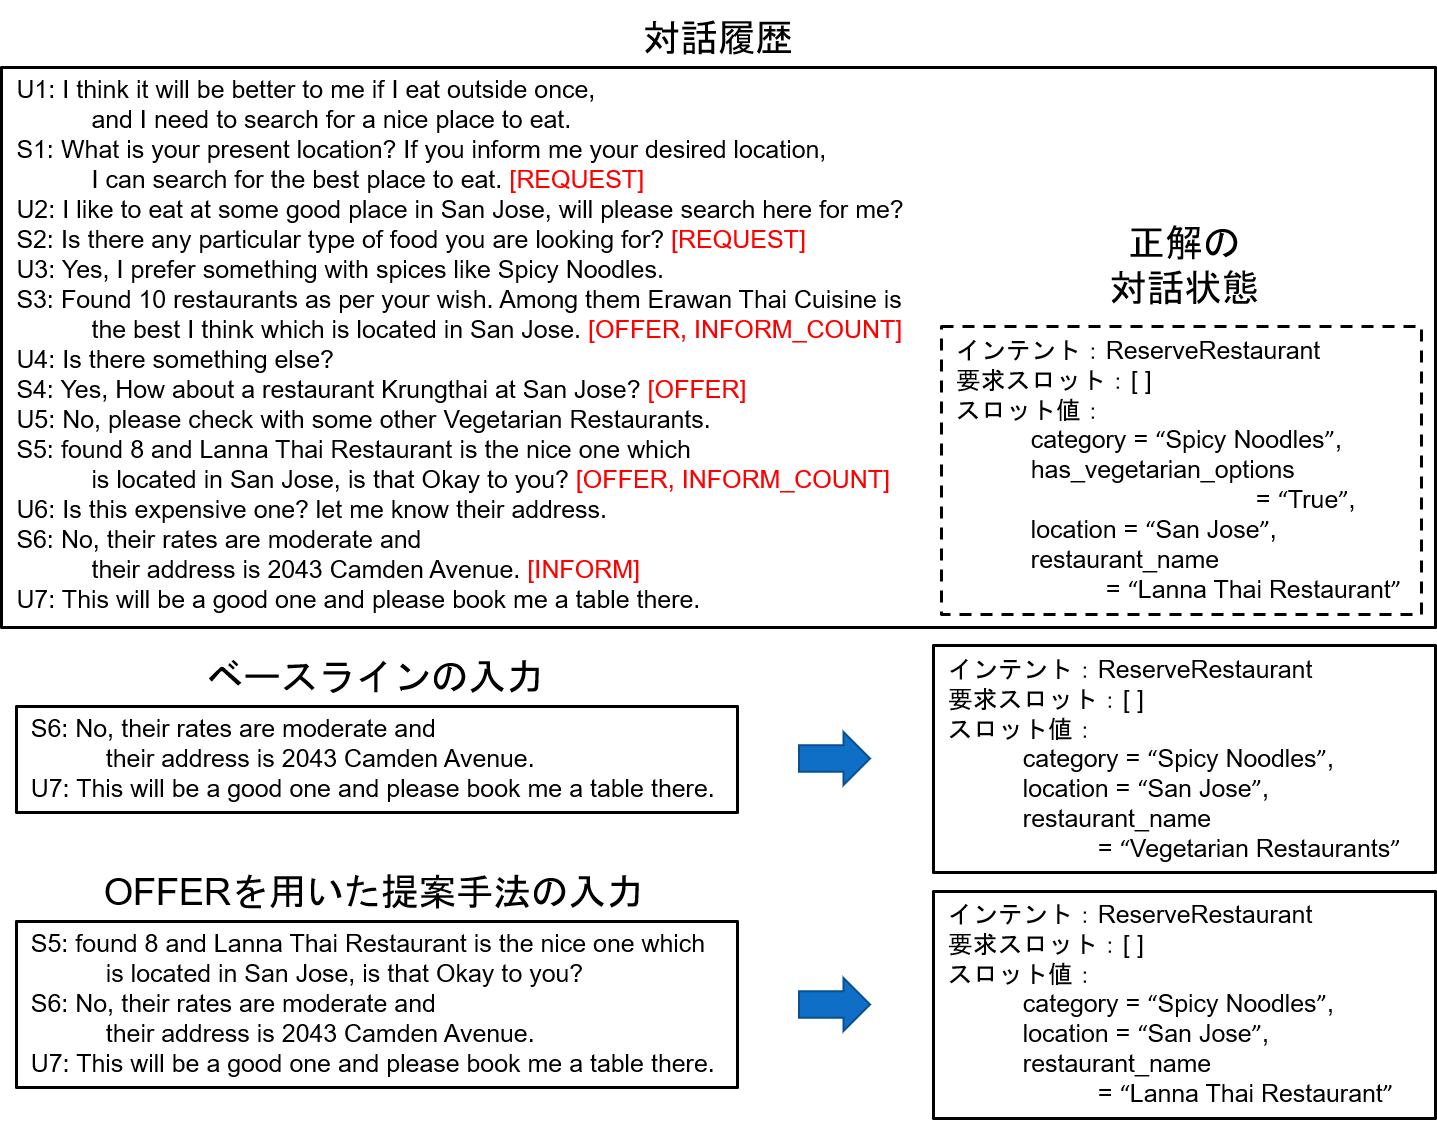
\includegraphics[width=15cm]{chapter6/case.eps}
    \caption{ベースラインとOFFERを用いた提案手法の出力結果}
    \label{fig:case}
\end{figure}

初めに,各対話行為タグを持つ発話がどの推定の性能を向上させるのかについて調べた.ベースラインモデルの結果と各対話行為タグで提案手法を行った際の結果を表\ref{tab:action_hikaku}に示す.Average Goal Accuracy をベースラインと比べると,“OFFER”が4.2\%, “INFORM\_COUNT”が 1.5\% 向上している.また,Joint Goal Accuracy をベースラインと比べると,“OFFER”が7.5\%, “INFORM\_COUNT”が 2.5\% 向上している.この結果は予備実験で示した通り,“OFFER” と “INFORM\_COUNT” を持つ発話が対話状態に反映されるスロット値候補を多く与えることと,図\ref{fig:case} に示したように過去の発話に存在するスロット値を推定可能になるからである.図\ref{fig:case} では“INFORM\_COUNT” でもレストラン名を推定できるが,“OFFER” と共存しない場合も存在するため,5.0\% の差が生まれている.他の対話行為の Average Goal Accuracy や Joint Goal Accuracy はベースラインと大差ないか減少しているため,スロット値推定に与える影響が少ない,もしくはその対話行為の発話がノイズとなっていると考えられる.また,図\ref{fig:case}では,候補ありスロットの“has\_vegetarian\_options”が推定できていない.このスロットは学習時に扱わない未知のスロットである.本研究では,未知のスロットや候補ありスロットに関しての対策を行っていないため,これらのスロット値推定の精度は向上していない.
\par

次に,Active Intent Accuracy をベースラインと比べると,“CONFIRM”が1.4\%, “OFFER”が1.1\%, “NOTIFY\_SUCCESS”が1.0\% 向上しているなど多くの対話行為で精度の向上が見られる.インテント推定はユーザの目的を推定しているので,対話の流れをより良く理解できる発話を履歴として入力できれば精度の向上が見込まれる.ゆえに,過去の発話を用いて情報量を増やした提案手法がベースラインの結果を超えている.ただし,対話の終わりに用いられる対話行為である“GOODBYE”は,対話の途中で抽出することはできないので精度が向上しなかった.また,インテント推定での誤りの多くは,最初の発話で異なるインテントを選択する誤りとインテントを維持すべきところで変更してしまう誤りであった.維持すべきところで変更してしまう誤りに関しては,前のターンのインテントをインテント推定の入力に用いることで解決すると期待できる.
\par
Requested Slot F1 に関しては大きな変化が見られない.つまり,要求スロットは現在のターンのユーザ発話の情報に大きく依存し,対話履歴では推定に必要な情報量があまり増加しない.
\par
ここまでの結果から,対話履歴をシステムの対話行為を用いて抽出することで性能が上がることを確認できた.今回は対話行為を 1 つだけ選択したが,複数の対話行為を用いることで更なる性能の向上が期待できる.

\begin{table}[thb]
    \centering
    \caption{従来手法との比較}
    \vspace{3mm}
    \label{tab:history_hikaku}
    \begin{tabular}{|c|r|r|r|r|r|} \hline
        &
        \begin{tabular}{c}
            Active \\ 
            Intent \\
            Accuracy
        \end{tabular} &
        \begin{tabular}{c}
            Requested \\
            Slot F1
        \end{tabular} &
        \begin{tabular}{c}
            Average \\ Goal \\ Accuracy
        \end{tabular} &
        \begin{tabular}{c}
            Joint \\ Goal \\ Accuracy
        \end{tabular} &
        \begin{tabular}{c}
            学習 \\ 時間
        \end{tabular} \\ \hline
        \begin{tabular}{c}
            ベースライン\\( 直近2発話\\入力 )
        \end{tabular} & 0.940 & 0.944 & 0.816 & 0.502 & 15.3(h)\\ \hline
        \begin{tabular}{c}
            提案手法 \\( OFFER )
        \end{tabular}
        & 0.946 & 0.947 & 0.845 & 0.565 & 20.7(h) \\ \hline
        直近3発話入力 & 0.943 & 0.947 & 0.815 & 0.508 & 20.9(h) \\ \hline
        直近4発話入力 & 0.974 & 0.948 & 0.844 & 0.553 & 26.3(h)\\ \hline
    \end{tabular}
\end{table}

続いて,従来の対話履歴の使用法との比較を行った.今回は提案手法として,他の対話行為より総合的に優れた結果を残した “OFFER” を用いた提案手法と,直近の2発話を入力としたモデル,3発話を入力としたモデル,4発話を入力としたモデルとを比較した.その結果を表\ref{tab:history_hikaku}に示す.ベースラインと提案手法の結果はミニバッチサイズを下げたことで変化している.直近3発話入力ではベースラインと比べて少ししか性能が向上していない.原因としては,1つ前のユーザ発話に含まれる既に推定済みの情報が現在のターンのユーザ発話に含まれる新しい情報の推定の妨げとなったことと,直近3発話では対話の流れを捉えるには情報不足であったことが考えられる.Joint Goal Accuracy に関しては,“OFFER”を用いた提案手法が直近3発話入力より5.7\% 高い数値を示している.同じ発話数でも性能が向上していることから,“OFFER”を用いた履歴抽出がスロット値推定に必要な情報を抽出できていることが分かる.また,提案手法は直近4発話入力よりJoint Goal Accuracyが1.2\% 高い数値を示している.これは,提案手法が対話によって6発話前や8発話前のスロット値も推定可能だからである.提案手法は3発話入力で直近4発話入力以上の結果を示していることから,対話状態追跡に重要な発話だけを抽出して重要ではない発話を取り除いているといえる.また,提案手法は直近4発話入力に比べて学習時間が5.4時間短く,計算量の削減にも成功している.しかし,Active Intent Accuracy では,直近4発話入力の方が提案手法に比べて 2.8\% 高い数値を示している.インテント推定は対話の流れを理解する必要があるため,連続した発話を入力する方が良い.そのため,提案手法のように過去の発話を抽出したものを用いると対話が断片的になり,連続した発話を入力とする従来手法より対話の流れを理解しにくいのだと考えられる.